\chapter{LITERATURE REVIEW}

\section{Literature Review}

\noindent The area of Handwritten Text Recognition (HTR) has witnessed an enormous shift from the tedious process of manual feature engineering to the era of deep learning, and now, to the era of advanced Transformer-based models. Initial attempts in digitizing Nepali handwriting scripts often encountered roadblocks due to the script's structural complexities. Dense compound character sets, floating vowel modifiers (matras), and the highly unpredictable nature of cursive handwriting are some of the challenges.

\noindent A significant milestone was reached with the advent of Convolutional Neural Networks (CNNs), as these networks are capable of learning and extracting such complex features \cite{baral2019handwritten, ghimire2020nepali, acharya2022nepali}. Although CNNs proved to be highly efficient in recognizing individual spatial patterns, they faced a structural limitation in incorporating the sequential patterns and long-range dependencies necessary for smooth reading of connected words. This, in turn, led to the natural progression toward sequence-to-sequence models and, consequently, Transformers. Using the self-attention mechanism, Transformers are able to bypass the need for a recurrent structure, as they can consider the entire context of a word. In fact, Vision Transformers and TrOCR models are currently achieving state-of-the-art results, proving to be highly efficient in modeling the complex visual geometry of low-resource languages like Nepali \cite{li2023trocr, hasan2023optical, li2025htr}.

\subsection{CNN-based Handwriting Recognition}
CNNs were undoubtedly a huge step forward for HTR, as they circumvented the need for feature extraction and instead learned hierarchical spatial features on their own. For example, Baral had built a good foundation with a CNN-based system that was specifically designed for isolated word recognition in Nepali scripts \cite{baral2019handwritten}. Ghimire et al. had also further improved this by optimizing the preprocessing steps to be better suited for handling Devanagari scripts \cite{ghimire2020nepali}, and Acharya et al. had also used similar CNN approaches for converting handwritten Nepali scripts to digital text \cite{acharya2022nepali}. However, there was a catch. While these models were extremely effective for isolated word recognition, standard CNNs did not possess the ``memory" that is often required for handling global dependencies in connected handwriting. This meant that it was extremely sensitive to the stylistic variations in handwriting.

\subsection{Sequence Modeling and Indic Script OCR}
To overcome the blind spots of CNNs on the word level, naturally, the solution was to resort to sequence modeling. For instance, Michael et al. demonstrated how important sequence-to-sequence models can be in cases where you have to directly map unsegmented image data to output text \cite{michael2019evaluating}.

\noindent When we consider the Indic scripts in more detail, the early Nepali-based OCR systems heavily relied on hybrid approaches that combined template matching and feature extraction. However, these were perfectly adequate for simple and well-structured characters but failed miserably when it came to the complex and non-uniform compound characters. The greatest barrier to deeper sequential learning was the absence of data. Gongidi and Jawahar alleviated this problem to some extent by introducing the IIIT-HW-Dev dataset and providing the long-awaited benchmark for Devanagari word-level OCR \cite{10.1007/978-3-030-86337-1_30}. Following this, Lalitha et al. attempted to explore new approaches that could improve the accuracy of Indic HTR systems, further supporting the claim that cursive Devanagari needs highly robust models \cite{10.1007/978-3-031-93688-3_17}.

\subsection{Vision Transformers for Handwritten Text}
Transformers have revolutionized the way we think about handwriting recognition. They have rewritten the rules. It began with Dosovitskiy et al.'s \cite{dosovitskiy2020image} Vision Transformer (ViT) model, which showed it is possible to process image patches with self-attention mechanisms and achieve superior performance compared to traditional convolutional networks. This is something we have seen being applied in handwriting recognition. In fact, Parres and Paredes \cite{parres2023fine} used vision-based encoder-decoder models to recognize complex, cursive scripts in historical documents. On the other hand, Yajima et al. \cite{yajima2024text} used Vision Transformers to recognize text in images and also classify script styles. More recently, Li et al. \cite{li2025htr} took it to another level with HTR-VT, which uses Vision Transformers in conjunction with sharpness-aware minimization to achieve state-of-the-art performance. In fact, across the board, comprehensive reviews of handwriting recognition models \cite{article} indicate that Transformer models are the new gold standard in extracting text from images.

\subsection{TrOCR and End-to-End Recognition}
A pivotal innovation in the field is the development of TrOCR by Li et al.~\cite{li2023trocr}. This architecture utilizes pre-trained models for both image and text modalities in an end-to-end fashion. The significance of TrOCR lies in its removal of complex CNN backbones and the reliance on Connectionist Temporal Classification (CTC) loss functions, opting instead for pure self-attention and cross-attention mechanisms. The flexibility of this model has been demonstrated in diverse applications, such as the handwriting pattern recognition research conducted by Adeli Shamsabad and Suen~\cite{inproceedings}. 

\noindent For low-resource languages, Hasan et al. proposed a Transformer-based model specifically designed for Nepali and Bengali OCR, achieving significant accuracy improvements with a reported Word Error Rate (WER) of 0.15~\cite{hasan2023optical}. Despite these strides, a notable research gap remains in the adoption of highly compressed, localized TrOCR variants. Specifically, the integration of a custom, lightweight BERT-based decoder engineered to address the unique phonetic and morphological nuances of the Devanagari script has yet to be fully explored for the Nepali language. This study seeks to address this gap.

\subsection{Role of Language Models and Custom Decoders in HTR}
While Vision Transformers excel at extracting spatial and structural features from word images, the ultimate accuracy of an end-to-end HTR system is heavily dependent on the decoder's capacity for sequence modeling~\cite{michael2019evaluating}. In TrOCR-style architectures, the decoder functions as a language model, generating character sequences based on visual embeddings and the linguistic context of the target language~\cite{li2023trocr}. Standard TrOCR implementations often utilize pre-trained English models like RoBERTa, which may not adequately capture the complexities of Indic scripts.

\noindent In the Devanagari script, relying exclusively on visual features can result in ambiguity, particularly when distinguishing between visually similar characters or tightly packed conjuncts~\cite{ghimire2020nepali}. By employing a localized, script-specific language model such as a custom-configured BERT decoder, it is possible to leverage the statistical probability of character co-occurrence in Nepali. Fine-tuning such a decoder specifically for Devanagari text~\cite{hasan2023optical, 10.1007/978-3-030-86337-1_30} provides the linguistic intuition necessary to correct visual misclassifications, representing a critical optimization pathway that this project investigates.

\newpage

\section{Related Theories}
\subsection{Optical Character Recognition (OCR)}

OCR is a technology that detects and converts printed or handwritten text found in digital images into machine-encoded, editable text. OCR systems combine hardware and software to transform physical documents into formats that computers can process and search. The most widely known application of OCR
is converting scanned paper documents into editable word-processor files. Modern OCR pipelines typically consist of four stages: image acquisition,preprocessing, character or word recognition, and post-processing. Handwritten text recognition is a particularly challenging subfield of OCR because writing
styles, stroke widths, and character spacing vary enormously across individuals.

\begin{figure}[h]
  \centering
  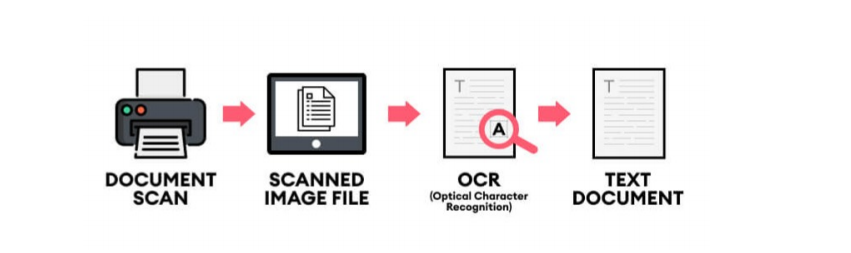
\includegraphics[width=0.75\textwidth]{img/ocr.png}
  \caption{General OCR Pipeline}
  \label{fig:ocr}
\end{figure}

\subsection{Traditional Approaches to OCR}

\subsubsection{Matrix Matching}
Matrix Matching was one of the earliest techniques used in OCR systems. An input character image is partitioned into a fixed grid and each cell is mapped to a pixel value, forming a matrix. This matrix is then compared against a library of pre-stored character templates using a similarity measure.While effective for clean, uniformly typeset text, matrix matching degrades sharply when character fonts, sizes, or orientations deviate from the stored templates, making it unsuitable for handwritten scripts such as Devanagari.

\subsubsection{Structural and Feature-Based Methods}
Structural analysis methods decompose a character into its constituent strokes,loops, junctions, and endpoints. Recognition is achieved by matching thesestructural primitives against a grammar or rule set that defines each character class. Feature-based methods extract statistical descriptors such as zonal
densities, projection profiles, and moment invariants from a segmented character image and feed them into classical classifiers (e.g., $k$-NN, SVM,or random forest). These methods offer better tolerance to font variation than matrix matching but still require explicit character segmentation, which is
problematic for connected or cursive scripts.

\subsubsection{Deep Learning-Based OCR Methods}

Neural networks have become the dominant paradigm for modern OCR because they can learn hierarchical feature representations directly from raw pixel data without manual feature engineering.

\subsubsection{Convolutional Neural Networks (CNNs)}

CNNs process input images through successive convolutional, pooling, and activation layers that progressively extract spatial features. Given an input
image $\mathbf{x}$, a convolutional layer applies a bank of learnable filters
$\mathbf{w}_k$:

\begin{equation}
  \mathbf{f}_k = \mathbf{x} * \mathbf{w}_k + b_k
\end{equation}

\noindent Pooling layers (max or average) then downsample the resulting feature maps,
reducing spatial dimensions while retaining dominant activations. The
Rectified Linear Unit (ReLU) is the standard non-linearity:

\begin{equation}
  \text{ReLU}(x) = \max(0,\, x)
\end{equation}

\noindent Fully connected layers at the top of the network produce a probability
distribution over character classes via a softmax output. For isolated
character recognition CNNs excel, but recognising full words or lines of text
requires a sequential component to capture inter-character context.

\begin{figure}[h]
  \centering
  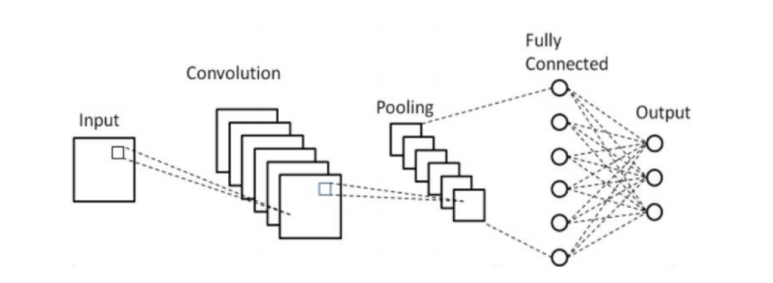
\includegraphics[width=0.7\textwidth]{img/cnn.png}
  \caption{Generalised Block Diagram of a CNN Model}
  \label{fig:cnn}
\end{figure}

\subsubsection{Recurrent Neural Networks and Long Short-Term Memory}

Recurrent Neural Networks (RNNs) extend feed-forward networks to handle
sequential data by maintaining a hidden state $h_t$ that is updated at each
time step $t$:

\begin{equation}
  h_t = \sigma\!\left(W_h\, h_{t-1} + W_x\, x_t + b\right)
\end{equation}

Plain RNNs suffer from vanishing and exploding gradients when sequences are
long. Long Short-Term Memory (LSTM) networks address this by introducing
gated memory cells. The update equations are:

\begin{align}
  f_t &= \sigma\!\left(W_f [h_{t-1}, x_t] + b_f\right) \\
  i_t &= \sigma\!\left(W_i [h_{t-1}, x_t] + b_i\right) \\
  \tilde{c}_t &= \tanh\!\left(W_c [h_{t-1}, x_t] + b_c\right) \\
  c_t &= f_t \odot c_{t-1} + i_t \odot \tilde{c}_t \\
  o_t &= \sigma\!\left(W_o [h_{t-1}, x_t] + b_o\right) \\
  h_t &= o_t \odot \tanh(c_t)
\end{align}
\noindent where $f_t$, $i_t$, $c_t$, and $o_t$ denote the forget gate, input gate,
cell state, and output gate respectively; $\odot$ denotes element-wise
multiplication. In handwriting recognition, LSTM networks are commonly
stacked bidirectionally (BiLSTM) so that each output position aggregates
context from both past and future time steps.

\subsubsection{Connectionist Temporal Classification (CTC)}

When a CNN-LSTM encoder produces a sequence of frame-level feature
vectors and the corresponding label sequence is shorter (as is typical for word
images), alignment between input frames and output characters is unknown
during training. CTC resolves this by marginalising over all possible
alignments. Given input length $T$ and target sequence $\mathbf{y}$ of length
$L$, CTC introduces a blank token $\varnothing$ and defines the loss as the
negative log-likelihood summed over all valid alignments $\pi$:

\begin{equation}
  \mathcal{L}_{\text{CTC}} = -\ln \sum_{\pi \,:\, \mathcal{B}(\pi) = \mathbf{y}}
  \prod_{t=1}^{T} p\!\left(\pi_t \mid \mathbf{x}\right)
\end{equation}
\noindent where the collapsing function $\mathcal{B}$ removes repeated characters and
blanks. CTC enables end-to-end training of sequence-to-label models without
requiring frame-level annotations.

\subsubsection{Transformer Architecture}

The Transformer is built entirely on
self-attention and dispenses with recurrence. Given an input sequence of
vectors $\mathbf{Z} \in \mathbb{R}^{n \times d}$, the scaled dot-product
attention is:

\begin{equation}
  \text{Attention}(Q, K, V)
  = \text{softmax}\!\left(\frac{QK^\top}{\sqrt{d_k}}\right)V
\end{equation}

\noindent where $Q$, $K$, and $V$ are linear projections of $\mathbf{Z}$.
Multi-Head Attention (MHA) runs $h$ independent attention heads in parallel and
concatenates their outputs:

\begin{equation}
  \text{MHA}(Q,K,V) = \text{Concat}(\text{head}_1, \ldots, \text{head}_h)\,W^O
\end{equation}

\noindent Each Transformer block couples MHA with a position-wise feed-forward network
(FFN) and applies layer normalisation with residual connections, enabling
gradient flow through very deep networks.

\subsubsection{Vision Transformer (ViT)}

The Vision Transformer (ViT) adapts the
Transformer encoder to image inputs by treating the image as a sequence of
non-overlapping patches. An image of size $H \times W$ is divided into
$N = HW / P^2$ patches of size $P \times P$ pixels. Each patch is flattened
and linearly projected to a $d$-dimensional embedding:

\begin{equation}
  \mathbf{z}_0 = [\mathbf{x}_{\text{cls}};\,
                  \mathbf{x}^1_p E;\; \mathbf{x}^2_p E;\; \ldots;\;
                  \mathbf{x}^N_p E] + \mathbf{E}_{\text{pos}}
\end{equation}

\noindent where $E \in \mathbb{R}^{(P^2 \cdot C) \times d}$ is the patch embedding
matrix and $\mathbf{E}_{\text{pos}}$ is a learnable positional encoding.
The sequence $\mathbf{z}_0$ is then processed by $L$ standard Transformer
encoder layers. Self-attention across patch tokens allows the model to capture
both local stroke features and long-range spatial relationships, which is
particularly beneficial for recognising structurally complex scripts like
Devanagari/Nepali.

\subsection{TrOCR: Transformer-Based OCR}

TrOCR \cite{li2023trocr} is an end-to-end transformer-based OCR model
that frames text recognition as an image-to-sequence problem. It follows
a standard encoder-decoder architecture in which the encoder extracts
visual features from the input image and the decoder autoregressively
generates the corresponding text sequence.

\begin{figure}[H]
  \centering
  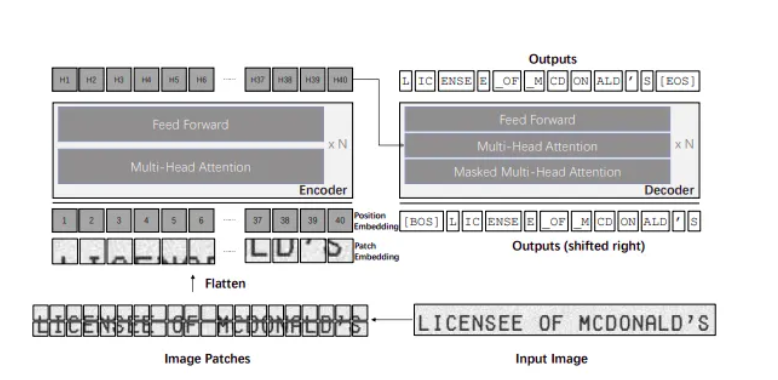
\includegraphics[width=0.80\textwidth]{img/theory.png}
  \caption{TrOCR Architecture}
  \label{fig:trocr}
\end{figure}

\subsubsection{Encoder}
The encoder is a Vision Transformer (ViT) that processes the input
image by first dividing it into a fixed grid of non-overlapping patches.
Each patch is linearly projected into a dense embedding vector, and
learnable position embeddings are added to retain spatial information.
The resulting sequence of patch embeddings is passed through a stack of
Transformer encoder layers, each comprising multi-head self-attention
and a position-wise feed-forward network. The output is a sequence of
contextual hidden states that collectively represent the visual content
of the image.

\subsubsection{Decoder}
The decoder is an autoregressive Transformer that generates the output
text one token at a time. It is initialised with a beginning-of-sequence
token \texttt{[BOS]} and continues generating tokens until the
end-of-sequence token \texttt{[EOS]} is produced. Each decoder layer
consists of three components: masked multi-head self-attention over
previously generated tokens, multi-head cross-attention over the encoder
hidden states, and a position-wise feed-forward network. At each
decoding step $t$, the model computes a probability distribution over
the vocabulary conditioned on all previously generated tokens and the
encoder output $\mathbf{H}$:
\begin{equation}
  p(y_t \mid y_{<t},\, \mathbf{H})
  = \text{softmax}\!\left(W_o\,
    \text{TransformerDecoder}(y_{<t},\, \mathbf{H})\right)
\end{equation}
The model is trained by minimising the cross-entropy loss over the full
target sequence:
\begin{equation}
  \mathcal{L} = -\sum_{t=1}^{T} \log p\!\left(y_t \mid y_{<t},\,
  \mathbf{H}\right)
\end{equation}
Both the encoder and decoder are initialised from large pre-trained
models, allowing TrOCR to leverage rich visual and linguistic
representations prior to task-specific fine-tuning.


\subsection{Dataset: IIIT-HW-Dev}

The IIIT Handwritten Devanagari (IIIT-HW-Dev) dataset
provides segmented word images of handwritten Devanagari script along with their Unicode ground-truth transcriptions. The dataset contains samples from multiple writers, covering a diverse vocabulary of Hindi/Nepali words. Eachimage has been pre-segmented at the word level, making it suitable for
word-image-to-text recognition without requiring additional line or word segmentation. The dataset is split into standard training, validation, and test partitions used throughout this work.

\subsubsection{Challenges of Devanagari Handwriting}

Devanagari/Nepali script presents several unique challenges for OCR:

\begin{itemize}
  \item \textbf{Conjunct consonants (half-characters):} Two or more consonants may combine into a single ligature, visually distinct from the base characters.
  \item \textbf{Matras (vowel diacritics):} Vowel signs attach above,below, or beside the base consonant, changing the visual appearance of the character significantly.
  \item \textbf{Headline (Shirorekha):} Most characters share a
horizontal headline stroke, causing characters within a word to be visually connected, complicating segmentation-based methods.
  \item \textbf{Inter-writer variability:} Stroke width, slant, and
    character proportions vary greatly across writers.
\end{itemize}

\noindent The end-to-end encoder-decoder approach adopted in this project directly
addresses these challenges by operating at the word-image level and relying on
the attention mechanism to learn character boundaries implicitly, without any
explicit segmentation step.

\newpage
\section{Review Matrix}



\setlength{\LTpre}{0pt}
\setlength{\LTpost}{0pt}
\renewcommand{\arraystretch}{1.3}
\noindent Table~\ref{tab:review-matrix} presents a summary of the literature reviewed in this chapter. It consolidates key studies, their methodologies, and contributions, providing a clear overview of the evolution of handwritten text recognition techniques.


\begin{longtable}[l]{|c|p{4.2cm}|c|p{3.5cm}|p{5cm}|}
\caption{Summary of Literature Review of NHWDTM system}
\label{tab:review-matrix} \\
\hline
\textbf{S.N.} &
\textbf{Title} &
\textbf{Year} &
\textbf{Algorithm} &
\textbf{Comments} \\ \hline
\endfirsthead

\multicolumn{5}{c}%
{\textbf{Table \thetable\ (continued)}} \\ \hline
\textbf{S.N.} &
\textbf{Title} &
\textbf{Year} &
\textbf{Algorithm} &
\textbf{Comments} \\ \hline
\endhead

% \hline \multicolumn{5}{r}{\textit{Continued on next page}} \\ \hline
\endfoot
\hline
\endlastfoot

1 & Handwritten Nepali character recognition and narration system \cite{baral2019handwritten} & 2019 & CNN & Built a foundational model to identify isolated Nepali characters, bypassing manual feature extraction. \\ \hline

2 & Evaluating sequence-to-sequence models for handwritten text recognition \cite{michael2019evaluating} & 2019 & Seq2Seq Models & Proved that sequence modeling is absolutely critical for mapping unsegmented image data directly to text. \\ \hline

3 & Nepali handwriting recognition using convolution neural network \cite{ghimire2020nepali} & 2020 & CNN, ANN & Optimized preprocessing stages to better handle the structural quirks of Devanagari scripts. \\ \hline

4 & An image is worth 16x16 words: Transformers for image recognition at scale \cite{dosovitskiy2020image} & 2020 & Vision Transformer (ViT) & Introduced ViT, proving self-attention on image patches could outperform traditional convolutions. \\ \hline

5 & iiit-indic-hw-words: A Dataset for Indic Handwritten Text Recognition \cite{10.1007/978-3-030-86337-1_30} & 2021 & Dataset Creation & Cleared a major data hurdle by providing a much-needed benchmark for Devanagari word-level OCR. \\ \hline

6 & Nepali handwritten character recognition system \cite{acharya2022nepali} & 2022 & CNN & Successfully utilized CNNs to convert handwritten Nepali text into an editable digital format. \\ \hline

7 & TrOCR: Transformer-based optical character recognition with pre-trained models \cite{li2023trocr} & 2023 & TrOCR (ViT + RoBERTa) & Introduced a brilliant end-to-end architecture that stripped away complex CNN backbones and CTC loss functions. \\ \hline

8 & Optical text recognition in Nepali and Bengali: A transformer-based approach \cite{hasan2023optical} & 2023 & Transformers & Achieved a massive leap in accuracy (WER of 0.15) for low-resource Indic scripts compared to traditional methods. \\ \hline

9 & Fine-tuning vision encoder-decoder transformers for historical documents \cite{parres2023fine} & 2023 & Vision Encoder-Decoder & Demonstrated the adaptability of vision encoder-decoder models on highly complex, cursive historical handwriting. \\ \hline

10 & Text detection and style classification from images Using ViT and transformer decoder \cite{yajima2024text} & 2024 & ViT, Transformer Decoder & Utilized Vision Transformers effectively to detect text and classify varied writing styles. \\ \hline

11 & HTR-VT: Handwritten text recognition with vision transformer \cite{li2025htr} & 2025 & ViT, SAM & Hit state-of-the-art results by combining Vision Transformers with sharpness-aware minimization. \\ \hline

12 & Automated Handwriting Pattern Recognition for mutlti-level personality classification using transformer ocr \dots Using TrOCR \cite{inproceedings} & 2025 & TrOCR & Showcased TrOCR's incredible adaptability for complex automated handwriting pattern classification tasks. \\ \hline

13 & Transforming images into words: optical character recognition solutions for image text extraction \cite{article} & 2025 & Comprehensive Review & Reinforced that Transformer architectures are the undeniable new gold standard for image text extraction. \\ \hline

14 & Enhancing Accuracy in Indic Handwritten Text Recognition \cite{10.1007/978-3-031-93688-3_17} & 2026 & Deep Learning / HTR & Explored crucial new techniques to handle cursive Devanagari, reinforcing the need for sequence-aware architectures. \\ \hline
\end{longtable}

